\documentclass[pra, twocolumn]{revtex4}


%%%%%%%%%%%%%%%%%%%%%%%%%%%%%%%%%%%%%%%%%%%%%%%%%%%%%%%%%%%%%%%%%%
%% Submetido ao       em XX/xx/2015             %%%
%%%%%%%%%%%%%%%%%%%%%%%%%%%%%%%%%%%%%%%%%%%%%%%%%%%%%%%%%%%%%%%%%%

\usepackage{float}
\usepackage[utf8]{inputenc}
\usepackage[brazil]{babel}
\usepackage{amsmath}% equation formatting
\usepackage{amssymb}% equation formatting
\usepackage{graphicx}% eps files
\usepackage{color}
\usepackage{subfigure}
\usepackage{epstopdf}
\usepackage{multirow}

%\usepackage{xcolor,colortbl}


\begin{document}

\title{Simula\c{c}\~ao do protocolo BB84 de criptografia qu\^antica utilizando um feixe laser intenso}

\author{A.L.P. Camargo$^{1,3}$, L.O. Pereira$^{1}$, W.F. Balthazar$^{2}$ J.A.O. Huguenin$^{1,3}$\footnote{Corresponding author. Email: huguenin@if.uff.br}}


\affiliation{$^1$Instituto de Ci\^encias Exatas, Universidade Federal Fluminense,\\ 
27213-145 Volta Redonda - RJ, Brazil}
\affiliation{$^2$Instituto Federal de Educa\c{c}\~ao, Ci\^encia e Tecnologia do Estado do Rio de Janeiro, Campus Volta Redonda,\\
27215-350 Volta Redonda - RJ, Brazil.}
\affiliation{$^3$Programa de P\'os Gradua\c{c}\~ao em F\'isica, Instituto de F\'isica,Universidade Federal Fluminense,\\
24210-346 Niter\'oi - RJ, Brazil.}




\begin{abstract}

Neste trabalho apresentamos um experimento muito simples explorando polariza\c{c}\~ao de um feixe laser intenso para simular a distribui\c{c}\~ao de uma chave criptogr\'afica atrav\'es do protocolo $BB84$ de criptografia qu\^antica. Nossa proposta est\'a baseada na analogia entre graus de liberdade de um feixe laser com estados qu\^anticos da luz, muito discutida atualmente. A proposta utiliza duas bases de polariza\c{c}\~ao linear, que \'e o ingrediente original do protocolo proposto por Bennet e Brassard. Dessa forma, o experimento permite um entendimento direto do princ\'ipio de funcionamento do protocolo. O experimento pode ser realizado em laborat\'orios did\'aticos dos cursos de gradua\c{c}\~ao em F\'isica e Engenharias bem como em espa\c{c}os de divulga\c{c}\~ao cient\'ifica. Al\'em disso, os resultados mostram que o experimento apresenta um ambiente muito prop\'icio para discuss\~ao sobre a diferen\c{c}a entre propriedades cl\'assicas e qu\^anticas da luz.\\


We present a very simple experiment exploring the polarization of an intense laser beam in order to perform an emulation of a cryptographic key distribution by the well known BB84 protocol. Our work relies on the analogy between classical degrees of freedom of a laser beam and quantum states, very discussed nowadays. Our analogue of a key distribution is made by using two polarization basis, the original ingredient used by Bennet and Brassard, which allow us a direct understanding of the protocol. The experiment can be performed in didactic laboratories or can be demonstrated in a classroom. In addition, the results show a very proper ambient to discuss the difference between classical and quantum measurement of light.

\end{abstract}


\maketitle

\section{Introdu\c{c}\~ao}

Em mundo cada vez mais digital \'e preciso confiar nos canais de transmiss\~ao de informa\c{c}\~ao. A criptografia moderna \'e baseada na distribui\c{c}\~ao de chaves criptogr\'aficas (uma longa sequ\^encia de zeros e uns - 0 e 1). Para encriptar uma mensagem digital (tamb\'em uma sequ\^encia de zeros e uns) que se deseja enviar em segredo, deve-se utilizar t\'ecnicas seguras de encripta\c{c}\~ao. Uma delas \'e a conhecida t\'ecnica "\textit{One-Time pad}"\cite{otp}, onde bits da mensagem s\~ao combinados com os bits da chave criptogr\'afica em uma opera\c{c}\~ao modular. Uma nova sequ\^encia bin\'aria ser\'a produzida com significado inintelig\'ivel para quem interceptar. Este procedimento \'e seguro desde que a chave seja rand\^omica e secreta. O receptor da mensagem tamb\'em deve possuir a chave criptogr\'afica de modo a recuperar a mensagem original procedendo tamb\'em uma opera\c{c}\~ao modular. A mensagem encriptada pode ser enviada em um canal p\'ublico n\~ao seguro desde que a chave seja partilhada apenas entre o rementente e o destinat\'ario. Logo, o problema da comunica\c{c}\~ao segura \'e a distribui\c{c}\~ao de chaves criptogr\'aficas. Atualmente, a t\'ecnica mais utilizada \'e o protocolo RSA \cite{rsa} que usa a distribui\c{c}\~ao p\'ublica de chaves, cuja seguran\c{c}a \'e baseada na dificuldade de fatora\c{c}\~ao de n\'umeros muito grandes. No futuro, computadores qu\^anticos, contudo, prometem uma velocidade de processamento muito superior a alcan\c{c}ada com computadores cl\'assicos, colocando em risco a seguran\c{c}a do processo de criptografia atual. 

De fato, a \'area de computa\c{c}\~ao e informa\c{c}\~ao qu\^antica tem recebido muita aten\c{c}\~ao de pesquisadores no que diz respeito a avan\c{c}os tecnol\'ogicos. Os resultados prometidos geram curiosidade e muita busca por informa\c{c}\~oes sobre o tema entre estudantes e interessados no assunto. Por este motivo, v\'arios trabalhos que buscam apresentar as ideias b\'asicas da \'area para este p\'ublico t\^em sido publicados \cite{iq1,iq2, iq3}. Para al\'em da difus\~ao do conhecimento cient\'ifico e tecnol\'ogico, o tema permite discutir fundamentos da f\'isica qu\^antica a n\'ivel de gradua\c{c}\~ao \cite{luiz}, enriquecendo o ensino desta importante \'area da F\'isica.

Uma das aplica\c{c}\~oes mais conhecidas da teoria qu\^antica  \'e a criptografia qu\^antica. Um protocolo alternativo, explorando propriedades qu\^anticas em estados de polariza\c{c}\~ao da luz, foi proposto em 1984 por Bennett e Brassard \cite{bb841}. Trata-se do conhecido protocolo $BB84$ de distribui\c{c}\~ao de chaves criptogr\'aficas, descrito detalhadamente na se\c{c}\~ao II deste trabalho. A realiza\c{c}\~ao experimental desta proposta foi pela primeira vez realizada pelo Laborat\'orio da IBM \cite{ibm}. O protocolo tamb\'em foi implementado com o envio de f\'otons em fibras sob o Lago de Genebra \cite{geneva}, al\'em de ter sido implementado na regi\~ao metropolitana de Boston\cite{darpa}.
%
Devido ao grande apelo tecnol\'ogico do protocolo $BB84$, surgiram trabalhos voltados \`a discuss\~ao did\'atica do protocolo de modo a promover um claro entendimento dos procedimentos e princ\'ipios f\'isicos envolvidos \cite{bb84RBEF}. Experimentos simples foram tamb\'em propostos de forma a mostrar a ess\^encia experimental do processo de distribui\c{c}\~ao de chaves pelo protocolo $BB84$. Usando posi\c{c}\~ao transversa e vari\'aveis de momento de um feixe laser por focaliza\c{c}\~ao, um experimento usando um circuito de \'otica linear demonstrou os princ\'ipios b\'asicos do protocolo\cite{lemelle}. Uma performance teatral muito divertida foi desenvolvida para ilustrar o funcionamento do protocolo $BB84$ usando bolas de chocolate embrulhadas em papel colorido e \'oculos de brinquedo com filtros de cor\cite{svozil}. Nestes experimentos, diferentes sistemas foram utilizados para representar os estados de polariza\c{c}\~ao de f\'otons e, atrav\'es destas representa\c{c}\~oes, a din\^amica do protocolo p\^ode ser discutida e compreendida.

No presente trabalho, estendemos a proposta de discutir informa\c{c}\~ao qu\^antica de forma b\'asica para o campo experimental. Apresentamos um experimento muito simples que pode ser implementado em laborat\'orios did\'aticos dos cursos de gradua\c{c}\~ao em F\'isica e Engenharias, utilizando a polariza\c{c}\~ao de um feixe laser intenso. Al\'em disto, pode ser realizado em espa\c{c}os de divulga\c{c}\~ao cient\'ifica para estudantes do ensino m\'edio e p\'ublico em geral. O experimento oferece uma vis\~ao direta do funcionamento do protocolo pois as codifica\c{c}\~oes dos bits que utilizamos s\~ao duas bases de polariza\c{c}\~ao de um feixe laser, os ingredientes originais do protocolo de Bennet e Brassard. A grande diferen\c{c}a reside na fonte luminosa empregada (no protocolo original \'e utilizada uma fonte de f\'otons \'unicos) e no sistema de detec\c{c}\~ao (uso de fotodetectores de avalanche no protocolo original). Vale destacar que propriedades do campo eletromagn\'etico cl\'assico tem sido utilizadas para simular protocolos qu\^anticos como jogos \cite{jogo1, jogo2}, portas l\'ogicas \cite{pgBras}, al\'em de violarem desigualdades an\'alogas \`a do regime qu\^antico como a desigualdade de Bell\cite{bellclass, nature}. As medidas em nosso experimento s\~ao feitas a partir da medida de intensidades de feixes intensos, que simulam os "clicks" relativos \`as medidas do protocolo original(fotocontagens). O experimento tamb\'em permite uma discuss\~ao muito direta e intuitiva da diferen\c{c}a entre os regimes cl\'assico e qu\^antico da luz, uma vez que a troca do feixe laser intenso por uma fonte de f\'otons \'unicos e a troca dos detectores levam ao regime original de realiza\c{c}\~ao do protocolo. Acreditamos que o experimento \'e um cen\'ario rico para a discuss\~ao sobre a descri\c{c}\~ao cl\'assica e qu\^antica da luz. Os resultados cl\'assicos do experimento podem ser contrapostos aos resultados esperados pela Mec\^anica Qu\^antica. Esta abordagem permitiu, ainda, simular experimentalmente um ataque de um espi\~ao e como o protocolo detecta sua presen\c{c}a.  

O trabalho est\'a esquematizado da seguinte forma: na se\c{c}\~ao II apresentamos uma descri\c{c}\~ao detalhada do protocolo $BB84$. A proposta experimental para simula\c{c}\~ao do protocolo e respectivo ataque de um espi\~ao \'e apresentada na se\c{c}\~ao III. Os resultados s\~ao apresentados e discutidos na se\c{c}\~ao IV. Por fim, as conclus\~oes do trabalho s\~ao sumarizadas na se\c{c}\~ao V.
   



\section{O protocolo BB84}
\label{bb84}

O protocolo BB84 foi desenvolvido para distribui\c c\~ao segura de chaves cirpitogr\'aficas utilizando estados qu\^anticos de polarização de f\'otons \'unicos.  A seguir, faremos a apresenta\c c\~ao da proposta original do protocolo e o efeito da a\c c\~ao de espionagem.

\subsection{Proposta original}
\label{origprop}

Uma vis\~ao esquem\'atica do protocolo \'e apresentada na Fig.\ref{basis}. A informa\c c\~ao come\c ca a ser transmitida por Alice, que envia f\'otons polarizados para Bob, que ir\'a medir a polariza\c c\~ao dos f\'otons enviados. Eles devem escolher entre duas bases, cada uma composta de dois estados ortogonais de polariza\c c\~ao --- a base $HV$ (polariza\c c\~ao horizontal e vertical) e a base  $+-$ (polariza\c c\~ao a $\pm 45^\circ$).

A base $HV$ \'e definida em rela\c c\~ao ao eixo de polariza\c c\~ao horizontal. Dessa maneira, um f\'oton com polariza\c c\~ao de  $0^\circ$ em rela\c c\~ao \`a horizontal tem polariza\c c\~ao $H$, e, analogamente, a polariza\c c\~ao que faz um \^angulo de $90^\circ$ com rela\c c\~ao \`a horizontal representa a polariza\c c\~ao $V$. A base $+-$ \'e definida da seguinte forma: as polariza\c c\~oes $\pm 45^\circ$, em rela\c c\~ao \`a horizontal, representam, respectivamente, os estados $+$ e $-$.

A codifica\c c\~ao dos bits \'e feita de maneira arbitr\'aria. Neste trabalho usaremos a seguinte conven\c c\~ao: o bit $0$ ser\'a a polariza\c c\~ao $H$ ou $+45^\circ$ e o bit $1$, a polariza\c c\~ao $V$ ou $-45^\circ$. Como podemos observar, para definir a polariza\c c\~ao de um bit precisamos primeiramente saber em qual base ele \'e preparado.

\begin{figure} [H]
     \centering
     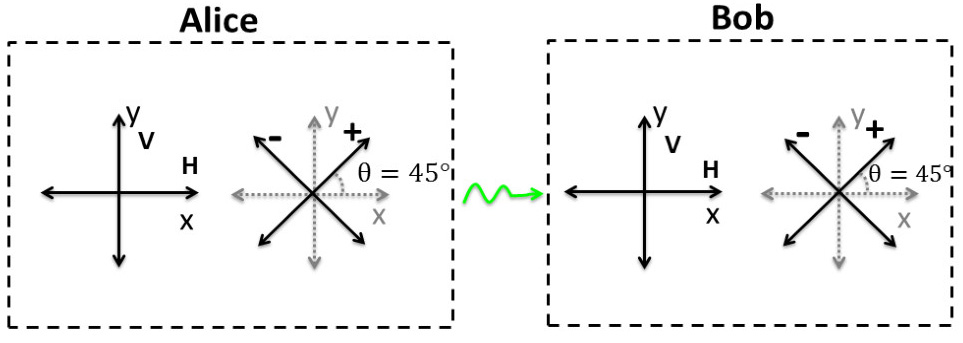
\includegraphics[scale=0.5,trim=0cm 5cm 0cm 4cm, clip=true,width =8.5 cm, height=3.8 cm]{fig1.jpg}
     \caption[Vis\~ao esquem\'atica do protocolo BB84.]{Vis\~ao esquem\'atica do protocolo BB84. Alice pode escolher tanto a base $HV$ quanto a $+-$. Para o primeiro caso, o bit $0$ \'e representado pela polariza\c c\~ao $H$ e o bit $1$ \'e representado pela polariza\c c\~ao $V$; enquanto que para o segundo caso, $0$ e representado por $+45^\circ$ e $1$ por $-45^\circ$. Bob faz apenas uma escolha: em qual das duas bases ir\'a medir o f\'oton.}
     \label{basis}
\end{figure}

Agora, iniciaremos a descri\c c\~ao do envio de bits. Primeiramente, Alice deve escolher uma base e um bit para enviar a Bob, enquanto Bob precisa escolher a base na qual ir\'a medir o bit recebido. Estas ``escolhas'' s\~ao totalmente aleat\'orias. Ap\'os o envio de um grande n\'umero de bits, Alice divulga publicamente a sequ\^encia de bases sorteadas que ela usou para preparar os bits enviados. Com isso, Bob compara a sequ\^encia de bases usadas por ele e mant\'em apenas as bases coincidentes, descartando todos os bits provenientes de medidas em bases que  n\~ao coincidiram com as bases que Alice usou no preparo. \'E importante notar que Alice publica apenas as bases da sequ\^encia enviada por ela, os bits equivalentes n\~ao s\~ao publicados. Para ver se a distribui\c c\~ao foi segura, ap\'os a filtragem das bases, eles comparam uma parte dos bits enviados e medidos e computam a porcentagem de acerto. \'E de se esperar, neste caso em que Bob mediu na mesma base que Alice enviou, que ele obtenha o mesmo bit. Por\'em, normalmente, parte dos bits podem ser rotacionados durante sua transmiss\~ao ou at\'e mesmo medidos de forma incorreta por Bob devido a desalinhamentos entre as bases. Por conta dessas circunst\^ancias, h\'a uma esperada taxa de erro na porcentagem de acerto dos bits, que depende da qualidade do canal. Se, ap\'os computar a porcentagem, o erro for maior do que o esperado, podemos concluir que provavelmente houve uma fonte externa de erro na transmiss\~ao --- provavelmente devido a uma espionagem. Caso contr\'ario, a comunica\c c\~ao est\'a segura o suficiente e o resto dos bits poder\~ao ser usados como chave criptogr\'afica.



\begin{table}[H]
\centering
  \begin{tabular}{|p{1.9cm}|p{1.6cm}|p{1.7cm}|p{1.4cm}|} 
   \hline
  
 \multicolumn{2}{|c|}{Alice}&\multicolumn{2}{|c|}{Bob}\\
   \hline
     Base A  & bit A & Base B & bit B \\
   \hline

   $+-$ & $0 $ &  $HV$ & $0$  \\ \hline
      $\textcolor{blue}{\textbf{\textbf{+-}}}$ & $\textcolor{blue}{\textbf{\textbf{0}}}$ & $\textcolor{blue}{\textbf{\textbf{+-}}}$ & $\textcolor{blue}{\textbf{\textbf{0}}}$  \\ \hline
      $\textcolor{blue}{\textbf{HV}}$ & $\textcolor{blue}{\textbf{\textbf{1}}}$ & $\textcolor{blue}{\textbf{HV}}$ & $\textcolor{blue}{\textbf{1}}$  \\ \hline
      $HV$ & $1$ & $+-$ & $0$  \\ \hline
      $\textcolor{blue}{\textbf{\textbf{+-}}}$ & $\textcolor{blue}{\textbf{\textbf{1}}}$ & $\textcolor{blue}{\textbf{\textbf{+-}}}$ & $\textcolor{blue}{\textbf{\textbf{1}}}$  \\ \hline
         \end{tabular}
    \caption{Exemplo da chave criptogr\'afica obtida. Ap\'os a aplica\c c\~ao do protocolo, apenas os bits provenientes de bases coincidentes s\~ao usados (em azul), os demais s\~ao descartados.Base A (B) representa a base escolhida por Alice (Bob) para prepara\c c\~ao (medida) dos bits. O bit A (B)representa o bit enviado (medido) por Alice (Bob)}.
              \label{Tabela1}
      \end{table} 	
      
      
      A Tabela \ref{Tabela1} mostra um pequeno exemplo da distribui\c c\~ao de chaves. S\~ao mostrados as bases e os bits escolhidos por Alice, as bases escolhidas por Bob e os bits lidos por Bob. Os dados em azul s\~ao relativos aos bits aproveitados, os demais s\~ao descartados. Neste caso, ap\'os aplicarem o protocolo, Alice e Bob obtiveram a seguinte chave de bits: $011$.
      
      
      

\subsection{Interfer\^encia de um espi\~ao}
\label{spy}

	No caso de comunica\c c\~oes seguras, os protocolos podem sofrer ataques de espi\~oes. Para o protocolo $BB84$, foram propostos alguns poss\'iveis ataques \cite{attacks}. O ataque mais simples que pode ser feito
	\'e a intercepta\c c\~ao e o re-envio de f\'otons para Bob pelo espi\~ao. Vamos discutir o caso mais simples onde podemos ver como a mec\^anica qu\^antica fornece seguran\c ca. Para o caso de Eva (a espi\~a, do Ingl\^es \textit{eavesdrop}) espionar a comuni\c c\~ao entre Alice e Bob, primeiramente ela precisa absorver o bit enviado por Alice e medi--lo da mesma maneira que Bob faria. A fim de n\~ao causar suspeitas em Bob, Eva precisa de um novo bit para ser enviado a ele como se fosse vindo de Alice. Como o teorema da n\~ao -- clonagem da Mec\^anica Qu\^antica \cite{nilsen} n\~ao permite que seja feita uma c\'opia perfeita de estados qu\^anticos, Eva pode enviar somente estados preparados aleatoriamente, do mesmo jeito que Alice faz , ou, na melhor das hip\'oteses para Eva, fazer uma c\'opia imperfeita do bit de Alice \cite{impcloning}. De qualquer forma, o bit re-enviado por Eva n\~ao ter\'a correla\c c\~ao perfeita com o bit enviado por Alice. Quando Bob for computar a porcentagem de acertos ap\'os a aplica\c c\~ao do protocolo, haver\'a erros nos bits obtidos com as bases coincidentes. O erro ocorre em dois casos: quando Alice e Eva escolhem a mesma base, por\'em diferentes bits --- com certeza este caso gera erro, uma vez que Bob simplesmente ir\'a ler o bit oposto, ou ainda, quando elas escolhem bases diferentes. Neste caso, Bob vai medir o bit certo com 50\% de probabilidade, para o caso em que Eva enviou bits preparados aleatoriamente. Para o caso de clonagem imperfeita o erro ser\'a menor. Em ambos os casos, contudo, ocorre o surgimento de uma da taxa de erro pois j\'a estamos assumindo aqui que as bases de Alice e Bob s\~ao as mesmas, uma vez que j\'a aplicamos o protocolo. Para o caso ideal (fonte de f\'otons \'unicos e dete\c c\~ao perfeita dos f\'otons) essa taxa de erro aponta que houve uma espionagem. Na Tabela \ref{Tabela2}, podemos ver a mesma situa\c c\~ao representada na Tabela \ref{Tabela1}, entretanto, agora com os erros provocados pela presen\c ca de Eva, para o caso em que ela prepara o re-envio aleatoriamente. Diferentemente de antes, ap\'os aplicarmos o protocolo, as bases coincidentes de Alice e Bob nem sempre ter\~ao os bits coincidentes. Em azul temos os bits coincidentes e em vermelho os bits de bases coincidentes que n\~ao est\~ao de acordo com o esperado. Dessa maneira, esta chave n\~ao pode ser usada e uma nova dever\'a ser providenciada.
		
	Existem outros tipos de ataque que oferecem mais risco ao protocolo, sobretudo quando o regime ideal de realiza\c c\~ao n\~ao pode ser alcan\c cado, por exemplo, pela dificuldade de produzir-se f\'otons \'unicos. Em geral, se produz pulsos com um n\'umero $N$ grande de f\'otons e  Eva poderia pegar uma pequena por\c c\~ao destes f\'otons se ela tiver acesso a um sistema de detec\c c\~ao de alta efici\^encia. Este ataque \'e conhecido como divisor de n\'umero de f\'otons, explicado com detalhes na Ref.\cite{PNS}. Podemos citar outras estrat\'egias de ataques como a que explora a imperfei\c c\~ao do sistema de detec\c c\~ao de Bob \cite{FS} e a estrat\'egia conhecida como "Cavalo de Tr\'oia" ou ataque por inje\c c\~ao de luz \cite{CT}. N\~ao entraremos em detalhes destas estrat\'egias de ataque por estarem al\'em do escopo do presente trabalho.       

\begin{table}[h]
  \begin{center}
  \begin{tabular}{ |c|c|c|c|c|c|}
   \hline
   \ Base A & bit A & Base E & bit E & Base B & bit B \\
   \hline
       $+-$ & $0$ & $HV$ & $0$ & $HV$ & $0$  \\ \hline
      $\mathbf{\textcolor{red}{+-}}$ & \textbf{$\textcolor{red}{0}$} & ${+-}$ & ${1}$ & \textbf{$\textcolor{red}{+-}$} & \textbf{$\textcolor{red}{1}$}  \\ \hline
       \textbf{$\textcolor{blue}{HV}$} & \textbf{$\textcolor{blue}{1}$} & $HV$ & $1$ & \textbf{$\textcolor{blue}{HV}$} & \textbf{$\textcolor{blue}{1}$}  \\ \hline
       $HV$ & $1$ & $HV$ & $1$ & $+-$ & $0$  \\ \hline
       \textbf{$\textcolor{red}{+-}$} & \textbf{$\textcolor{red}{1}$} & $+-$ & $0$ & \textbf{$\textcolor{red}{+-}$} & \textbf{$\textcolor{red}{0}$}  \\ \hline
   \end{tabular}
       \caption{Exemplo da influ\^encia de um espi\~ao na distribui\c c\~ao de chaves criptogr\'aficas. Ap\'os a aplica\c c\~ao do protocolo, nem todos os bits coincidiram. Em vermelho, os bits provenientes de bases coincidentes que apresentam erro. A, E e B representam Alice, Eva e Bob, respectivamente. No caso de Eva, mostramos as bases e bits enviados a Bob.}
        \label{Tabela2}
  \end{center}
  \end{table} 	



\section{Experimento}

Nossa proposta \'e realizar uma simula\c c\~ao do Protocolo BB84 usando um feixe laser polarizado cl\'assico, ou seja, em regime de feixe intenso. As bases escolhidas e a codifica\c c\~ao dos bits s\~ao exatamente as mesmas da proposta original:polariza\c c\~ao. Utilizamos a base $HV$ (polariza\c c\~ao $H$ correspondendo ao bit $0$ e polariza\c c\~ao $V$ correspondendo ao bit $1$) e a base $+-$ ($+45^\circ \rightarrow bit~ 0$ e $-45^\circ \rightarrow bit ~ 1$). As bases s\~ao definidas a partir do \^angulo de rota\c c\~ao de placas de meia onda ($PMO$), como veremos a seguir. Vale notar que a \'unica diferen\c ca entre o experimento deste trabalho e o protocolo original\'e o regime de intensidade da luz. No protocolo original \'e exigido regime de produ\c c\~ao e contagem de f\'otons \'unicos, enquanto nossa proposta did\'atica utiliza feixes intensos e mede fotocorrentes. 

\subsection{Montagem experimental livre de espi\~ao}\
\label{semEva}

A primeira parte do experimento simula a troca de uma chave criptogr\'afica entre Alice e Bob sem a interfer\^encia da espi\~a, ou seja, Eva n\~ao participa desta etapa do experimento (Se\c c\~ao \ref{origprop}). O esquema experimental est\'a esbo\c cado na Fig. \ref{exp1}. Um feixe laser horizontalmente polarizado passa atrav\'es da primeira placa de meia onda, denominada $PMO_{\theta_A} $, que \'e usada por Alice com o objetivo de escolher suas bases de prepara\c c\~ao e os bits que ser\~ao enviados a Bob. \'E importante notar que Alice ajusta sua base e seu bit apenas fazendo uma rota\c c\~ao  $\theta_A$ do eixo r\'apido da $PMO$ em rela\c c\~ao \`a horizontal (dire\c c\~ao da polariza\c c\~ao incidente). Para a base $HV$, ela usa $\theta_A = 0^\circ$ para enviar o feixe na polariza\c c\~ao $H$ (bit $0$) e $\theta_A = 45^\circ$ para enviar o feixe na polariza\c c\~ao $V$ (bit $1$). Para a base $+-$, ela usa  $\theta_A = 22.5^\circ$ para enviar o feixe na polariza\c c\~ao $+45^\circ$ (bit $0$) e $\theta_A = -22.5^\circ$ para polariza\c c\~ao $-45^\circ$ (bit $1$). 

\begin{figure} [H]
     \centering
     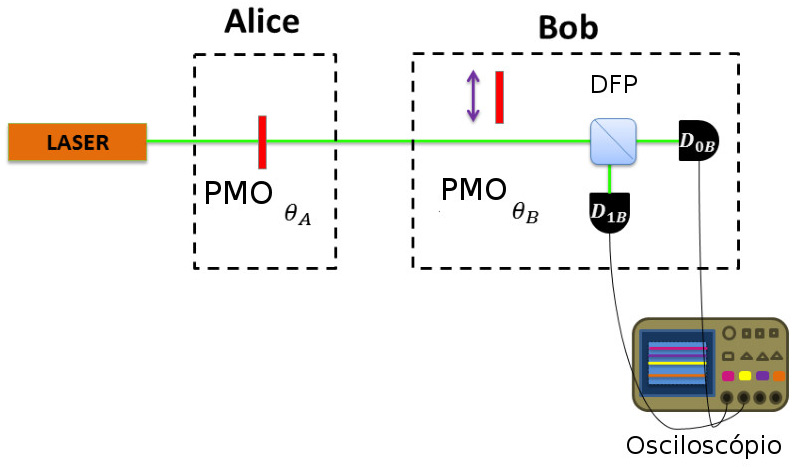
\includegraphics[scale=0.7, trim=3cm 1cm 1cm 3cm, clip=true,width =8.5 cm, height=5 cm]{fig2.jpg}
     \caption[Esquema experimental da primeira parte do experimento, sem espionagem. ]{Esquema experimental da primeira parte do experimento. Alice pode escolher suas bases e bits a serem enviados usando uma \'unica placa de meia onda $PMO_{\theta_A}$. As medidas de Bob s\~ao feitas usando a meia onda $PMO_{\theta_B}$ e um $DFP$ (Divisor de Feixe Polarizado). As sa\'idas ``$0$'' e ``$1$'' s\~ao captadas pelos detectores $D_{0B}$ e $D_{1B}$ e registrados pelo oscilosc\'opio digital.}
     \label{exp1}
\end{figure}

Como Bob apenas realiza as medidas dos bits, ele precisa escolher apenas em qual base ser\~ao feitas essas medidas. Para isso, ele utiliza um Divisor de Feixes Polarizado ($DFP$) que transmite a polariza\c c\~ao $H$ e reflete a polariza\c c\~ao $V$. Dois detectores s\~ao utilizados (um em cada sa\'ida do $DFP$) monitorando simultaneamente atrav\'es de um oscilosc\'opio digital a intensidade obtida em cada uma delas. NA aus\^encia de oscilosc\'opios podemos utilizar mult\'imetros para leitura das fotocorrentes.

Portanto, Bob mede na base $HV$ utilizando o $DFP$ e detectores em cada sa\'ida. Se Alice manda o bit $0$ na base $HV$ (polariza\c c\~ao $H$), apenas a componente transmitida pelo $DFP$ ter\'a uma parcela significativa de intensidade  no detector  $D_{0B}$. Para o bit $1$ (polariza\c c\~ao $V$), apenas a componente refletida ser\'a medida pelo detector $D_{1B}$. No caso onde Alice manda seus bits na base $+-$ (polariza\c c\~ao $\pm 45^\circ$) o $DFP$ ir\'a projetar estas polariza\c c\~oes na base $HV$, de forma que os dois detectores ir\~ao registrar intensidades pr\'oximas (balanceadas). Com isso, para este experimento, podemos concluir que quando as intensidades est\~ao registrando valores pr\'oximos em ambos detectores, significa que Bob escolheu uma base diferente de Alice. Pode-se usar alguma estrat\'egia para leitura desta medida, como por exemplo, ler o bit correspondente a maior intensidade, mesmo que seja apenas um pouco maior. N\~ao nos preocuparemos com estes resultados, uma vez que estes casos ser\~ao descartados.  

Para que Bob me\c ca na base $+-$, ele precisa mapear os estados da base $+-$ em estados da base $HV$ e medir com o $DFP$. Isto \'e feito inserindo-se uma placa de meia onda, $PMO_{\theta_B}$, com o a\^ngulo $\theta_B =22.5^\circ$ em rela\c c\~ao \`a horizontal imediatamente antes do $DFP$. Se Alice mandar o bit $0$ na base $+-$ ( polariza\c c\~ao $+ 45^\circ$), o feixe laser passa pela $PMO_{\theta_B=22,5^\circ}$ e sua polariza\c c\~ao \'e rodada para a polariza\c c\~ao $H$. Com isso, o \'unico detector a captar o laser ser\'a o $D_{0B}$. Para o bit $1$ (polariza\c c\~ao $-45^\circ$), a $PMO_{\theta_B=22,5^\circ}$ rotaciona esta polariza\c c\~ao levando-a \`a polariza\c c\~ao $V$. Com isso, apenas o feixe refletido pelo $DFP$ ser\'a medido, pelo detector $D_{1B}$. Ou seja, para medir na base $+-$, \'e suficiente introduzir uma meia onda $HWP_{\theta_B=22,5^\circ}$ imediatamente antes do $DFP$. Note que quando Alice manda um bit na base $HV$, a $HWP_{\theta_B}$ transforma a polariza\c c\~ao em $\pm 45^\circ$ e os dois detectores apresentar\~ao intensidades balanceadas, mostrando uma escolha errada de base. Novamente a leitura de um bit poder ser feita tomando-se o que apresentar uma intensidade ligeiramente maior.

Com esta configura\c c\~ao \'e poss\'ivel simular o protocolo BB84. Primeiramente, \'e escolhido um n\'umero $N$ de bits que ser\~ao enviados. Usando um gerador de n\'umeros aleat\'orios gerados numericamente em um computador, s\~ao produzidas tr\^es sequ\^encias de $N=100$ n\'umeros inteiros, que s\~ao classificados como pares ou \'impares. A primeira sequ\^encia \'e usada para simular a escolha de base de Alice, onde os n\'umeros pares correspondem a base $HV$ e os n\'umeros \'impares correspondem a base $+-$. A segunda sequ\^encia \'e usada para a escolha do bit enviado por Alice, e n\'umeros pares correspondem ao bit $0$ e n\'umeros \'impares ao bit $1$. Finalmente, a terceira sequ\^encia representa a escolha de base a qual o Bob usar\'a para medir o bit --- que segue a mesma correspond\^encia feita para Alice. Ap\'os o t\'ermino do envio, Alice e Bob comparam suas bases e mant\'em apenas os bits cujas bases coincidiram. A chave ser\'a composta pelos bits enviados (lidos) por Alice (Bob) nas bases coincidentes. 






\subsection{Montagem experimental em presen\c ca de um espi\~ao}
\label{comEva}

A segunda parte do experimento, mostrado na Fig.\ref{exp2}, representa a distribui\c c\~ao de uma chave criptogr\'afica entre Alice e Bob com a presen\c ca da espi\~a, ou seja, Eva ir\'a interferir na comunica\c c\~ao (Se\c c\~ao \ref{spy}). Alice usa o seu feixe laser para enviar os bits usando o procedimento apresentado na Se\c c\~ao \ref{semEva}. Por\'em, em vez do feixe polarizado ir diretamente a Bob, Eva desvia o feixe para que possa med\'i-lo. Eva faz esta medida da mesma maneira que Bob mede um bit:  usando um $DFP$ e, alternadamente, uma $PMO_{\theta_{E_I}}$, de acordo com a base escolhida para medir. Como Eva absorve o bit enviado por Alice, ela precisa de uma fonte extra de bits para mandar para Bob. Vamos utilizar a estrat\'egia mais simples, em que Eva prepara aleatoriamente os bits a serem enviados, a partir de um novo feixe laser e uma segunda placa de meia onda $PMO_{\theta_{E_{II}}}$. Eva mede o bit enviado por Alice com os detectores $D_{0E}$ e $D_{1E}$. Finalmente, Bob mede o feixe que ele recebe, i.e., o feixe enviado por Eva. Desta vez, como h\'a duas medidas sendo feitas, o oscilosc\'opio de quatro canais (podem ser utilizados mult\'imetros) apresenta dois pares de resultados: o bit medido por Eva (enviado por Alice) e o bit medido por Bob (enviado por Eva).

Para esta etapa s\~ao produzidas tr\^es novas sequ\^encias de n\'umeros inteiros aleat\'orios que representam: a escolha da base de medida de Eva, sua base de preparo de bit e sua escolha de bit. Ap\'os o t\'ermino do envio de bits, Alice e Bob comparam suas bases e mant\'em os bits oriundos das medidas com a base coincidente. Para verificarem a confiabilidade do canal, usam parte da chave para investigar se houve alguma perturba\c c\~ao.


\begin{figure} [H]
     \centering
     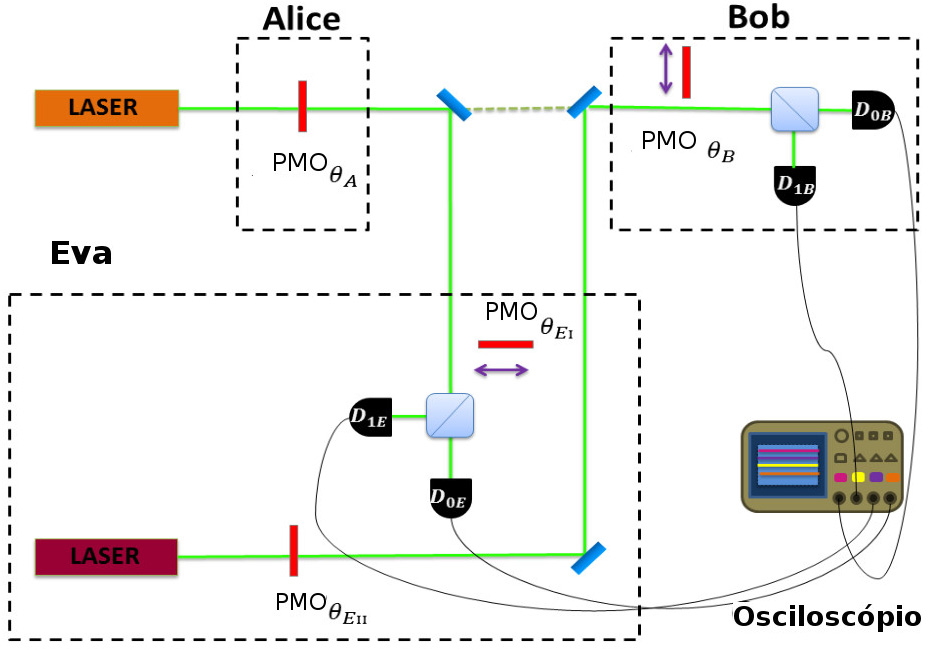
\includegraphics[scale=0.55, trim=0cm 1cm 1cm 0cm, clip=true,width =8.5 cm, height=5 cm]{fig3.jpg}
     \caption[Esbo\c co experimental da segunda parte do experimento, sem espionagem.]{Esbo\c co experimental da segunda parte do experimento. Alice e Eva escolhem suas bases e bits usando apenas uma \'unica placa de meia onda cada uma: ($PMO_{\theta_A}$ e $PMO_{\theta_E II}$). As medidas s\~ao feitas por Eva e Bob, usando respectivamente $PMO_{\theta_EI}$ junto com um $DFP$ e $PMO_{\theta_B}$ junto com outro $DFP$. Os bits $0$'s s\~ao detectados pelos detectores $D_{0B}$ e $D_{0E}$ e os $1$'s s\~ao detectados por $D_{1B}$ e $D_{1E}$, todos registrados pelo oscilosc\'opio digital.}
     \label{exp2}
\end{figure}

\section{Resultados e discuss\~oes}

Nesta se\c c\~ao apresentaremos os resultados da realiza\c c\~ao de cada experimento. Mostraremos casos particulares que ilustram o funcionamento do protocolo e a consolida\c c\~ao dos resultados experimentais. 

\subsection{Resultados para o protocolo sem a presen\c ca de espi\~ao}
\label{resultSemEva}

 Vamos discutir os resultados da primeira parte do experimento, na aus\^encia da espi\~a (Fig.\ref{exp1}). Para come\c car, quatro casos ser\~ao apresentados. O primeiro caso \'e quando Alice sorteia n\'umeros pares para a base e para o bit, ou seja, base $HV$ --- bit $0$ (polariza\c c\~ao $H$). Na sequ\^encia, Bob tamb\'em sorteia um n\'umero par, ou seja, ele mede na base $HV$ (apenas o $DFP$ ser\'a usado na medi\c c\~ao). O resultado obtido pelo oscilosc\'opio para esta situa\c c\~ao est\'a sendo mostrado na Fig.\ref{fig4}(a).

Neste caso, a polariza\c c\~ao $H$ \'e transmitida pelo $DFP$ e o detector $D_{0B}$ capta a intensidade mostrada no Canal 1 do oscilosc\'opio  ($CH1$ - tra\c co amarelo). O detector $D_{1B}$, mostrado no Canal 2 ($CH2$ - tra\c co azul), apresenta intensidade muito perto de zero, uma vez que a polariza\c c\~ao do feixe detectado \'e horizontal. Esse \'e o caso onde Alice e Bob coincidem suas bases. Um segundo caso  poss\'ivel \'e quando Bob, diferentemente do primeiro caso, sorteia um n\'umero \'impar para medir seu bit, ou seja, ele mede na base $+-$. Agora, ele usa a  $PMO_{\theta_B=22.5^\circ}$ antes do $DFP$ para realizar a medida. O resultado dessa medida, mostrado na Fig.\ref{fig4}(b),  apresenta uma intensidade distrubu\'ida entre os dois detectores $D_{0B}$ e $D_{1B}$, uma vez que a meia onda rotacionou a polariza\c c\~ao do laser para $+45^\circ$. Para operar a leitura de um bit nesta medida, podemos considerar como sendo bit $1$, uma vez que o Canal 2 (tra\c co azul) \'e ligeiramente superior.  

\begin{figure} [H]
     \centering
     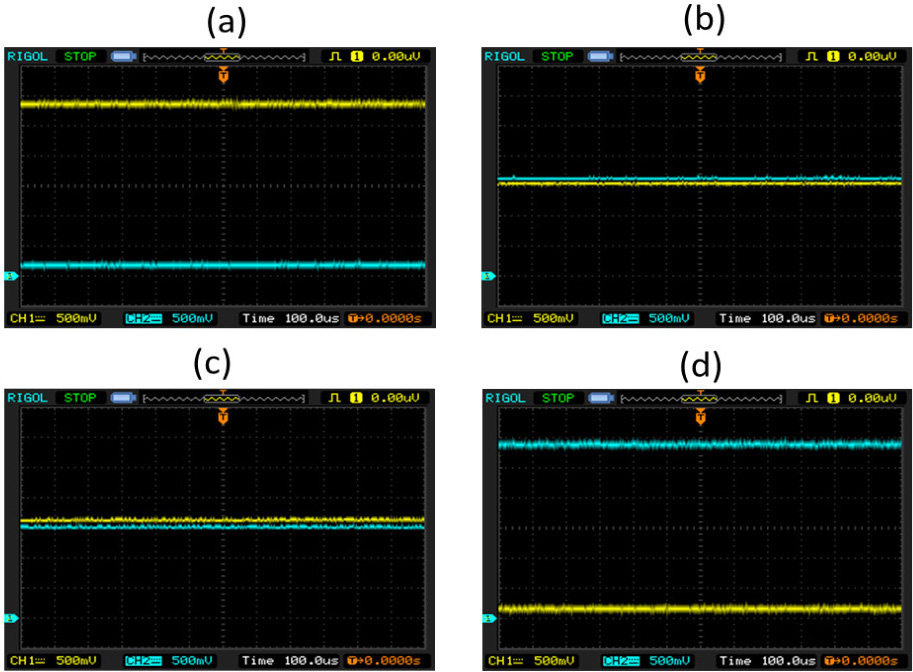
\includegraphics[scale=0.6, trim=1cm 0cm 1cm 0cm, clip=true,width =8.5 cm, height=6 cm]{fig4.jpg}
     \caption[Resultados obtidos pelo oscilosc\'opio de acordo com a configura\c c\~ao da Fig.\ref{exp1}]{Resultados obtidos pelo oscilosc\'opio de acordo com a configura\c c\~ao da Fig.\ref{exp1} para os seguintes casos: imagem (a) quando Alice envia bit $0$ na base $HV$ e Bob mede na base $HV$; imagem (b) Alice manda o bit $0$ na base $HV$ mas Bob mede na base $+-$; imagem (c) Alice manda o bit $1$ na base $+-$ e Bob mede na base $HV$; imagem (d) Alice manda o bit $1$ na base $+-$ e Bob mede na base $+-$.}
     \label{fig4}
\end{figure}

O terceiro caso \'e quando Alice sorteia dois n\'umeros \'impares, ou seja, ela manda o bit $1$ na base $+-$ (ajustando a meia onda em $\theta_A=+22.5^\circ$) e Bob sorteia um n\'umero par, medindo na base $HV$. A Fig.\ref{fig4}(c) mostra o resultado obtido nessa circunst\^ancia que, assim como o anterior, resulta em intensidades balanceadas nos detectores. Neste caso, como o Canal 1 apresenta intensidade um pouco maior, podemos realizar a leitura do bit $0$. Finalmente, o quarto caso acontece quando tanto Alice quanto Bob sorteiam n\'umeros \'impares. Ou seja, Alice manda o bit $1$ na base $+-$ e Bob mede na base $+-$. O feixe laser com polariza\c c\~ao $-45^\circ$ passa atrav\'es da  $HWP_{\theta_B=+22.5^\circ}$ e sua polariza\c c\~ao \'e convertida para a polariza\c c\~ao $V$. Com isso, o feixe \'e refletido pelo $DFP$ e o detector $D_{1B}$ capta a intensidade ($CH2$ - tra\c co azul) enquanto Canal 1 permanece praticamente sem intensidade, como mostra a Fig.\ref{fig4}(d).

Como pode ser observado, quando Alice e Bob coincidem suas bases, apenas um detector (o associado ao bit enviado por Alice) apresenta uma intensidade significativa. Em contrapartida, quando eles diferem em suas escolhas de base, ambos detectores apresentam intensidades, aproximadamente equivalentes.

\begin{table}[H]
\begin{center}
\begin{tabular}{|c|c|c|c|}
\hline
\multicolumn{2}{|c|}{Alice} & \multicolumn{2}{|c|}{Bob} \\ \hline
$B_{ENV}$  & $b_{ENV}$ & $B_{MED}$ & $b_{MED}$ \\ \hline
HV & 0 & $+-$ & $1$ \\ \hline
HV & 1 & $+-$ & $0$ \\ \hline
$+-$ & $0$ & $+-$ & $0$ \\ \hline
$+-$ & $1$ & $+-$ & $1$ \\ \hline
HV & 0 & $+-$ & $1$ \\ \hline
$+-$ & $1$ & $+-$ & $1$ \\ \hline
HV & 0 & HV & 1 \\ \hline
HV & 1 & $+-$ & $0$ \\ \hline
$+-$ & $1$ & $+-$ & $1$  \\ \hline
$+-$ & $0$ & $+-$ & $0$  \\ \hline
\end{tabular}
\end{center}
\caption{Amostra de 10 dos 100 bits enviados, de acordo com a configura\c c\~ao da Fig.\ref{exp1}, sem a participa\c c\~ao de Eva. $B$ e $b$ representam Base e bit medidos ($MED$) e enviados ($ENV$), respectivamente}
\label{tabela3}
\end{table}

 A Tabela III apresenta uma amostragem de 10 repeti\c c\~oes das 100 realizadas no experimento. \'E importante notar que na aus\^encia de Eva todas as vezes em que Alice e Bob usam a mesma base, Bob necessariamente acerta o bit.




\subsection{Resultados do experimento com a presen\c ca de espi\~ao}

Passamos agora a discutir os resultados relativos \`a segunda parte do experimento, quando Eva come\c ca a espionagem, de acordo com a configura\c c\~ao da Fig.\ref{exp2}. O mesmo procedimento apresentado na Se\c c\~ao IV-A \'e repetido. Por\'em, agora s\~ao gerados seis n\'umeros aleat\'orios para cada bit trocado correspondendo a: base de Alice, bit de Alice, base de medida de Eva, base de envio de Eva, bit de envio de Eva e base de medida de Bob. Tamb\'em foi usada a mesma quantidade de bits $N=100$. Apenas os n\'umeros referentes \`as escolhas de Eva foram gerados nesta etapa de forma que os n\'umeros relativos \`as escolhas de Alice e Bob foram mantidos iguais ao caso da se\c c\~ao \ref{resultSemEva}, para que, dessa maneira, a \'unica diferen\c ca nesta segunda parte do experimento fosse realmente a intromiss\~ao de Eva. Assim, temos Alice mandando os mesmos bits e Bob usando as mesmas bases para fazer as medidas. Entretanto, como Eva interfere no sistema, ser\'a poss\'ivel ver que o resultado n\~ao \'e preservado. Quando aplicado o protocolo, como visto anteriormente, s\~ao mantidos apenas os bits cujas bases coincidiram. Em vista disso, ser\'a discutido neste momento apenas estes dois casos. Na Fig \ref{imagem2}, cada coluna representa um dos casos em quest\~ao. No primeiro caso, Alice sorteia dois n\'umeros pares (bit $0$ - polariza\c c\~ao $H$), Eva tamb\'em sorteia dois n\'umeros pares para enviar seu bit  (bit $0$ - polariza\c c\~ao $H$), e Bob sorteia um n\'umero par para realizar a medida (medida na base $HV$). A imagem E-a) da Fig.\ref{imagem2} apresenta o resultado obtido por Eva neste processo (bit $0$ - polariza\c c\~ao $H$). \'E interessante notar que esta situa\c c\~ao \'e an\'aloga a situa\c c\~ao da Fig.4(a), por\'em agora em vez de Bob, Eva \'e quem esta detectando o bit. Dessa maneira, os resultados nos detectores s\~ao: $D_{0E}$ mede uma alta intensidade mostrada no Canal 1 ($CH1$ - tra\c co amarelo) e $D_{1E}$ quase n\~ao detecta intensidade muito baixa mostrada no Canal 2 ($CH2$ - tra\c co azul).

\begin{figure} [H]
     \centering
     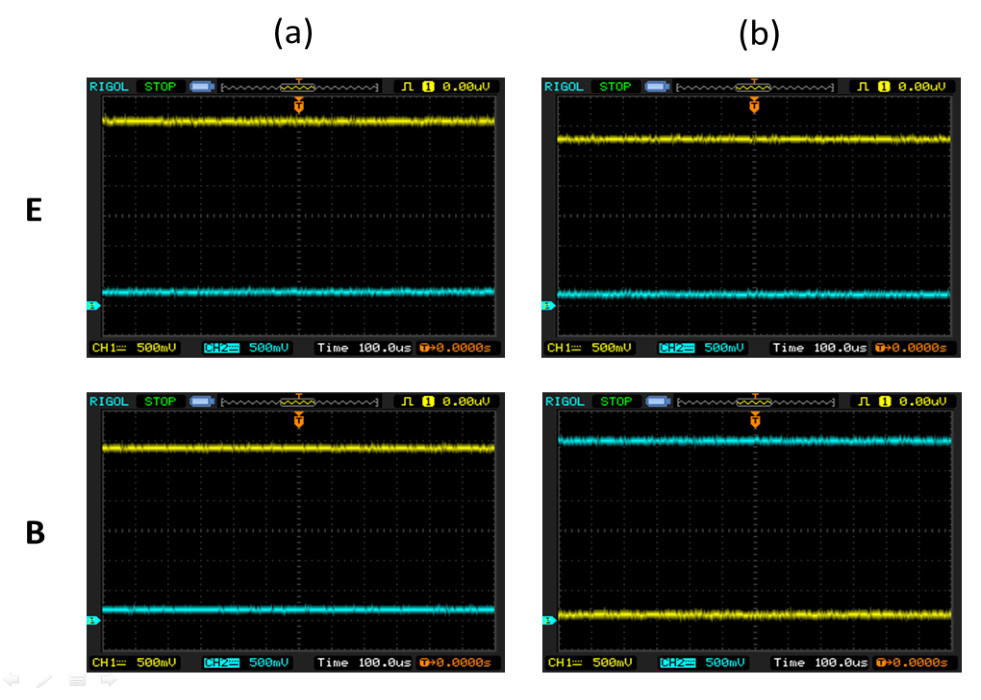
\includegraphics[scale=0.55, trim=0.7cm 0cm 0.7cm 0cm, clip=true,width =8.0 cm, height=5.5 cm]{fig5.jpg}
     \caption{Resultados obtidos pelo oscilosc\'opio de acordo com a configura\c c\~ao da Fig.\ref{exp2} para os seguintes casos: imagem E(a) Alice envia o bit $0$ na base $HV$ e Eva mede na base $HV$; imagem B(a) Eva manda o bit $0$ na base $HV$ e Bob mede na base $HV$; imagem E(b) Alice manda o bit $0$ na base $HV$ e Eva mede na base $HV$; imagem B(b) Eva manda o bit $1$ na base $HV$ e Bob mede na base $HV$.}
     \label{imagem2}
\end{figure}

Com isso, conclu\'imos que Alice e Eva coincidiram suas bases. A imagem B-a) da Fig. \ref{imagem2} apresenta o resultado obtido por Bob (bit $0$ - polariza\c c\~ao $H$). Pode-se observar que este resultado \'e an\'alogo ao anterior, ou seja, Eva e Bob coincidiram suas bases assim como Alice e Eva. Para concluir este primeiro caso, observa-se que apesar da presen\c ca de Eva, Bob acertou o bit enviado por Eva; por\'em, vale ressaltar que foi devido a coincid\^encia do bit enviado por Eva ser id\^entico ao enviado por Alice com a mesma base. Nem sempre acontecer\'a desta maneira como ser\'a visto a seguir.

No segundo caso Alice sorteia de novo dois n\'umeros pares (bit $0$ - polariza\c c\~ao $H$), Eva sorteia, respectivamente, um n\'umero par e um \'impar para enviar seu bit (bit $1$ - polariza\c c\~ao $V$), e Bob escolhe um n\'umero par (medida na base $HV$). A imagem E-b) da Fig.\ref{imagem2} apresenta o resultado obtido por Eva (bit $0$ - polariza\c c\~ao $H$), que \'e precisamente o mesmo resultado obtido por Eva anteriormente. Com isso conclui-se que Alice e Eva coincidiram suas bases novamente e consequentemente obtiveram o mesmo bit. A imagem B-b) mostra o resultado obtido por Bob (bit $1$ - polariza\c c\~ao $V$). A polariza\c c\~ao $V$ vinda de Eva \'e refletida pelo $DFP$ e o detector $D_{1B}$ capta quase toda a intensidade, mostrada no canal 2 do oscilosc\'opio ($CH2$ - tra\c co azul). O outro detector, $D_{0B}$ ($CH1$ - tra\c co amarelo), capta intensidade muito baixa, uma vez que a polariza\c c\~ao do laser est\'a totalmente vertical. Nesta circusnt\^ancia, Alice e Bob coincidiram suas bases; entretanto, Bob n\~ao acertou o bit enviado por Alice. Isto aconteceu devido a influ\^encia de Eva, uma vez que ela espionou a comunica\c c\~ao e mandou para Bob um novo bit totalmente aleat\'orio que desta vez n\~ao coincidiu como bit enviado por Alice. Por esta raz\~ao, o protocolo estabelece que Alice e Bob comparem uma pequena parte da chave criptogr\'afica. Se houve espionagem, eles ir\~ao observar um erro de bits muito alto para as bases coincidentes. A tabela IV apresenta uma amostra de 10 das 100 sequ\^encias feitas no laborat\'orio, que tem como \'unica diferen\c ca para o caso anterior o acr\'escimo das a\c c\~oes de Eva. Diferentemente da situa\c c\~ao anterior, quando Alice e Bob coincidirem suas bases, n\~ao necessariamente Bob obter\'a o mesmo bit enviado por Alice.



\begin{table} [H]
\begin{center}
\begin{tabular}{|p{1.0cm}|p{1.0cm}|p{1.4cm}|p{1.4cm}|p{1.4cm}|p{1.5cm}|}
\hline
\multicolumn{2}{|c|}{Alice} & \multicolumn{3}{|c|}{Eva} & \multicolumn{1}{|c|}{Bob} \\ \hline
{$B_{ENV}$} & {$b_{ENV}$} &  {$B_{MED}$} & {$B_{ENV}$} & {$b_{ENV}$} & {$B_{MED}$}\\ \hline
HV & 0 & $+-$ & $0$ & $+-$ & $0$\\ \hline
HV & 1 & HV & 1  & $+-$ & $1$ \\ \hline
$+-$ & $0$ & HV & 0 & $+-$ & $0$\\ \hline
$+-$ & $1$ & $+-$ & $0$ & $+-$ & $0$ \\ \hline
HV & 0 & $+-$ & $1$ & $+-$ & $1$ \\ \hline
$+-$ & $1$ & $+-$ & $0$ & $+-$ & $0$ \\ \hline
HV & 0 & $+-$ & $1$ & HV & 1\\ \hline
HV & 1 & $+-$ & $0$ & $+-$ & $0$ \\ \hline
$+-$ & $1$ & HV & 1  & $+-$ & $1$  \\ \hline
$+-$ & $0$ & $+-$ & $1$ & $+-$ & $1$ \\ \hline
\end{tabular}
\end{center}
\caption{Amostra de 10 dos 100 bits enviados de acordo com a configura\c c\~ao da Fig. 3, onde h\'a a participa\c c\~ao de Eva. $B$ e $b$ representam Base e bit medidos ($MED$) e enviados ($ENV$), respectivamente}
\label{tabela4}
\end{table}

Ap\'os as realiza\c c\~oes experimentais em ambas configura\c c\~oes, com e sem Eva, uma sumariza\c c\~ao dos resultados \'e apresentada na Tabela \ref{Tabela5}. Para a realidade deste trabalho, que \'e apenas uma simula\c c\~ao da distribui\c c\~ao de chaves, a taxa de erro \'e devido apenas a presen\c ca da espi\~a. Para concluir, nota-se que quando Eva n\~ao interfere na comuni\c c\~ao, ap\'os aplicar o protocolo, Alice e Bob v\~ao necessariamente acertar seus bits. Entretanto, quando Eva de fato interfere, eles v\~ao coincidir seus bits aproximadamente metade das vezes, que \'e precisamente a mesma chance de Eva mandar, por acaso, o mesmo bit enviado por Alice.


\begin{table} [H]
\centering
\begin{tabular}{|p{2.0cm}|p{2.0cm}|p{2.0cm}|p{2.0cm}|} 
  %\begin{tabular}{|c|c|c|c|}
   
   \hline
      & BC& bC & \% Acertos \\
   \hline

   Sem Eva & $49$ &  $49$ & $100.00'\%$  \\ \hline
   Com Eva & $49$ & $22$ & $44.90'\%$  \\ \hline
    
         \end{tabular}
    \caption{Resultados obtidos ap\'os a repeti\c c\~ao de $N=100$ bits enviados em ambas configura\c c\~oes: com e sem Eva. $BC$ corresponde a bases coincidentes e $bC$, bits coincidences.}
              \label{Tabela5}
      \end{table} 	


\section{Cl\'assico $\times$ Qu\^antico}

Como podemos ver, o experimento realizado simula o resultado da distribui\c c\~ao de chaves criptogr\'aficas pelo protocolo $BB84$ de criptografia qu\^antica. Qual a diferen\c ca deste experimento para a implementa\c c\~ao do protocolo? Basicamente, a fonte de luz envolvida e o sistema de detec\c c\~ao. Note que o protocolo descrito na Se\c c\~ao \ref{bb84} trabalha com a codifica\c c\~ao dos bits na polariza\c c\~ao de f\'otons individuais, e a seguran\c ca repousa no Teorema de N\~ao Clonagem\cite{nilsen}. Eva n\~ao consegue clonar o bit enviado por Alice para que ela possa mandar uma c\'opia perfeita para Bob. Se isto fosse poss\'ivel o protocolo n\~ao seria seguro.

A presente proposta usa exatamente as mesmas bases e interpreta\c c\~oes do protocolo original mas n\~ao pode ser usado para distribui\c c\~ao de chaves por quest\~ao de segura\c ca. Sendo os bits enviados em um feixe intenso, Eva poderia desviar uma pequena fra\c c\~ao do feixe, alguns poucos f\'otons se ela tem os recursos. Ao retirar esta pequena fra\c c\~ao Bob n\~ao seria capaz de distinguir a \ pequena diferen\c ca na intensidade, e n\~ao seria capaz de perceber a espionagem. 

Vale destacar que a vers\~ao qu\^antica de nosso experimento pode ser discutida de forma muito direta e traz a vantagem de gerar oportunidade para observarmos a diferen\c ca de comportamento nos regimes cl\'assicos e qu\^anticos, sendo uma ferramenta interessante para introdu\c c\~ao de conceitos chave da teoria qu\^antica. Para chegarmos \`a vers\~ao qu\^antica deste proposta, temos que primeiramente, trocar a fonte luminosa intensa (laser) por uma fonte de f\'otons \'unicos. Os detectores ($D_{0B}$ e $D_{1B}$) utilizados no experimento devem ser trocados por dois contadores de f\'otons
($CF_{0B}$ e $CF_{1B}$). Toda prepara\c c\~ao de bases e estados, bem como a \'otica utilizada para as medidas e leituras dos bits s\~ao id\^enticas \`as utilizados no caso de feixe intenso.

Para o caso qu\^antico sempre teremos um ``\textit{click}'' em um dos contadores de f\'otons. Para o caso em que as bases de Alice e Bob coincidem, apenas o $CF$ relativo ao bit enviado ir\'a ser acionado. No caso em que Alice e Bob n\~ao tiverem suas bases coincidindo, ao inv\'es das intensidades balanceadas observadas no caso cl\'assico, continuaremos  observando um \'unico $CF$ ser acionado, j\'a que n\~ao podemos dividir um f\'oton. Por exemplo, se Alice enviar o f\'oton com polariza\c c\~ao $+$ (base $+-$, bit $0$) e Bob medir na base $HV$, teremos uma probabilidade de $50\%$ do f\'oton ser transmitido no $DFP$ e detectado por $CF_{0B}$, e  $50\%$ de probabilidade de ser refletido pelo $DFP$ e ser detectado pelo $CF_{1B}$. Eis a fonte de erro intr\'insica do protocolo e o motivo pelo qual os bits medidos em bases n\~ao coincidentes s\~ao descartados da chave. Se repetirmos a medida do exemplo acima enviando muitos f\'otons, metade deles
ser\'a transmitida e metade refletida. Nosso experimento est\'a inteiramente de acordo com esta previs\~ao j\'a que apresenta intensidades balanceadas no caso de bases n\~ao coincidentes. Se tomarmos a intensidades $I_{jB}$ de cada detector $ D_{jB}$ ($j=0,1$) e a intensidade total $I_T$ (soma das intensidades), a raz\~ao $I_{jB}/I_T$ correspodenr\'a a probabilidade de um f\'oton ser detectado no detetor $D_{jB}$. De fato, para experimentos de \'optica linear, o resultado da m\'edia para $N$ repeti\c c\~oes do experimento qu\^antico coincide com o resultado de uma realiza\c c\~ao do experimento cl\'assico onde temos um n\'umero extremamente grande de f\'otons em um feixe de poucos miliwatts.  

Para o experimento na presen\c ca de um espi\~ao, o regime qu\^antico \'e alcan\c cado fazendo com que Eva tamb\'em tenha acesso \`a fontes de f\'otons \'unicos e contadores de f\'otons para sua detec\c c\~ao. 

\section{conclus\~oes}

 Neste trabalho propomos e realizamos experimentalmente um experimento simples para demonstrar os princ\'ipios de funcionamento do protocolo $BB84$ de criptografia qu\^antica em que foi explorado o mesmo instrumental para implementa\c c\~ao do protocolo original, ou seja, duas bases de polariza\c c\~ao da luz. Por\'em, utilizamos uma fonte de laser intensa, no regime cl\'assico. Nossos resultados mostram claramente todas as nuances do protocolo, inclusive a a\c c\~ao de um espi\~ao, o que n\~ao foi at\'e hoje explorado nas implementa\c c\~oes ilustrativas do protocolo. Uma discuss\~ao sobre as propriedades qu\^anticas do protocolo podem ser feita a partir de nossos resultados, que s\~ao uma ferramenta interessante para discutir as diferen\c cas entre os regimes cl\'assico e qu\^antico. Uma vers\~ao qu\^antica do nosso experimento pode ser obtida diretamente pela substitui\c c\~ao da fonte luminosa e dos detectores, levando o aparato \`a vers\~ao original do protocolo $BB84$.

\section*{Acknowledgement}
CNPq, FAPERJ, INCT- Informa\c c\~ao Qu\^antica

\begin{thebibliography}{99}

\bibitem{otp}{F. Rubina,``One-Time Pad cryptography,'' Cryptologia, \textbf{20}, 359–364, (1996).}


%A Method for Obtaining Digital Signatures and Public-Key Cryptosystems
\bibitem{rsa}{R.L. Rivest, A. Shamir, and L. Adleman,``A Method for Obtaining Digital Signatures and Public-Key Cryptosystems,'' Comm. of Tech ACM, \textbf{21}, 120:126, (1978).}

% 
\bibitem{iq1}{Jos\'e Roberto Castilho Piqueira, ``Teoria qu\^antica da informa\c c\~ao: impossibilidade de c\'opia,
entrela\c camento e teletransporte, Rev. Bras. Ensino de F\'is., v. 33, n. 4, 4303 (2011).}


%
\bibitem{iq2}{Jos\'e, Marcelo Archanjo, Piqueira, Jos'e Roberto Castilho and Lopes, Roseli de Deus, `` Introdu\c c\~ao \`a programa\c c\~ao qu\^antica, Rev. Bras. Ensino F\'is., vol.35, no.1, p.1-9 (2003).}

\bibitem{iq3}{ Cabral, Gustavo Eulalio M., Lima, Aércio Ferreira de and Lula Jr., Bernardo, ``Interpretando o algoritmo de Deutsch no interferômetro de Mach-Zehnder", Rev. Bras. Ensino Fís., v.26, no.2, p.109-116, (2004).}
%

\bibitem{luiz}{Davidovich, Luiz,``Os quanta de luz e a \'otica qu\^antica, Rev. Bras. Ensino F\'is., vol.37, no.4, p.4205-1-4205-12, (2015)}

%“Quantum cryptography: Public key distribution and coin tossing,” 
\bibitem{bb841}{C. H. Bennett and G. Brassard,``Quantum cryptography: Public key distribution and coin tossing,'' Proceedings of the IEEE International Conference on Computers, Systems, and Signal Processing, Bangalore,India IEEE Computer Society Press, 175–179, (1984). }


%“Experimental quantum cryptography,”
\bibitem{ibm}{C. H. Bennett, F. Bessette, G. Brassard, L. Salvail, and J. Smolin,``Experimental quantum cryptography,''  J. Cryptology 5, 3–28 (1992). }

%Automated "plug & play" Quantum Key Distribution
\bibitem{geneva}{ Grégoire Ribordy, Jean-Daniel Gautier, Nicolas Gisin, Olivier Guinnard, Hugo Zbinden, Electronics Letters, \textbf{34}, (22), 2116 - 2117 (1998).}

%“Current status of the DARPA quantum network,”
\bibitem{darpa} {C. Elliott, A. Colvin, D. Pearson, O. Pikalo, J. Schlafer, and H. Yeh,``Current status of the DARPA quantum network,'' quant-ph/0503058, (2005).}



%Introducao \`a criptografia qu\ˆantica
\bibitem{bb84RBEF}{ Gustavo Rigolin e Andr\'es Anibal Rieznik, Revista Brasileira de Ensino de F\'isica, v. 27, n. 4, p. 517 - 526, (2005).}



%A simple optical demonstration of quantum cryptography using transverse position and momentum variables
\bibitem{lemelle}{D. S. Lemelle, M. P. Almeida, P. H. Souto Ribeiro, and S. P. Walborn,``A simple optical demonstration of quantum cryptography using transverse position and momentum variables,'' Am. J. Phys. \textbf{74} ,542-547 (2006).}


%Staging quantum cryptography with chocolate balls
\bibitem{svozil}{Karl Svozil,``Staging quantum cryptography with chocolate balls,'' Am. J. Phys. \textbf{74}, 800-803,  (2006).}

\bibitem{jogo1} A.~R.~C.~Pinheiro, C.~E.~R. Souza, D.~P.~Caetano, 
J.~A.~O.~Huguenin, A.~G.~M.~Schmidt, and A.~Z.~Khoury, “Vector vortex implementation of a quantum game,"  J. Opt. Soc. Am. B {\bf 30}, 3210 (2013).


%
 \bibitem{jogo2} W. F. Balthazar, M. H. M. Passos, A. G. M. Schmidt, D. P. Caetano,and J. A. O. Huguenin, “Experimental realization of the quantum duel game using linear optical circuits," J. Phys. B 48, 165505 (2015).
 %
 
\bibitem{pgBras}{W. F. Balthazar, D. P. Caetano, C. E. R. Souza, and J. A. O. Huguenin,  "Using Polarization to Control the Phase of Spatial Modes for Application in Quantum Information",Brazilian Journal of Physics 44, 658 (2014).}


%Bell Carol
\bibitem{bellclass}{C. V. S. Borges, M. Hor-Meyll, J. A. O. Huguenin, and A. Z. Khoury,``Bell-like inequality for the spin-orbit separability of a laser beam,'' Phys. Rev. A \textbf{82}, 033833 (2010). }


%nature
\bibitem{nature}{K. H. Kagalwala, G. D. Giuseppe, A. F. Abouraddy, and B. E. A. Saleh,``Bell's measure in optivcal classical coherence,'' Nat. Photonics \textbf{7}, 72 (2012).}

%nature
\bibitem{attacks}{R. Aggarwal, H. Sharma, and D. Gupta,
``Analysis of Various Attacks over BB84 Quantum Key
Distribution Protocol,'' International Journal of Computer Applications \textbf{20}, 28-31 (2011).}


%QI
\bibitem{nilsen}{Michael A. Nielsen and Isaac L. Chuang, \textit{ Quantum Computation and Quantum Information} Cambridge University Press, (2000).}


\bibitem{impcloning}{V. Scarani, S. Iblisdir, N. Gisin, and Antonio Ac\`in, ``Quantum cloning,'' REVIEWS OF MODERN PHYSICS, \textbf{77}, 1225-1256 (2005).}


\bibitem{PNS}{N. Lu tkenhaus, ``Security against eavesdropping
attacks in quantum cryptography,'' Phys. Rev. A 54(1), 97-
111 (1996).}
 
\bibitem{FS}{V.  Makarov and D.R. Hjelme, ``Faked states attack on quantum cryptosystems,'' Journal of Modern Optics, \textbf{52}, 691-705 (2005).}
 

\bibitem{CT}{A. Vakahitov, V.  Makarov and D.R. Hjelme, ``Large
pulse attack as a method of conventional optical eavesdropping in quantum cryptography,'' Journal of Modern Optics, \textbf{48}, 2023-2038 (2001).}



\end{thebibliography}

\end{document}

